In the second part of this thesis, we consider the problem of memory management in a single router.
Modern routers consist of two logical components. Those two components use disjoint memory (often of distinct type) and disjoint processing units:
\begin{enumerate}
  \item The forwarding plane, which  contains forwarding table described in the previous section, and performs the actual packet transmission according to the forwarding table.
  \item The control plane, which is responsible for reflecting the network topology in the forwarding table.
\end{enumerate}

As highlighted in the introduction, the forwarding component has finite memory, and in an increasingly common scenario the size of forwarding table exceeds the size of available memory.
One of the solutions is to store only a part of a~forwarding table on the forwarding device, that acts as a cache for the complete forwarding table that is stored in the control plane, see Figure~\ref{fig:router}.
However, this might result in the situation, where the forwarding device does not have sufficient information to proceed.
We will show how to deal with this.

Note that the technical feasibility of our solution heavily depends on the
rule dependencies. In the most ubiquitous scenario, the rules are prefixes of
IP addresses (they are bit strings). Whenever a packet arrives, the router
follows a longest matching prefix (LMP) scheme: it searches for the rule that
is a~prefix of the destination IP of the packet and among matching rules it
chooses the longest one. In other words, if the prefixes corresponding to
rules are stored in the tree\footnote{We do not have to assume that they are
actually stored in a real tree; this tree is implicit in the LMP scheme.},
then the tree is traversed from the root downwards, and the last found rule is
used.

\section{Technical Setup}

This explains why we require the cached nodes to form a subforest:
leaving a less specific rule on the router while evicting a more specific one
(i.e., keeping a~tree node in cache while evicting its descendant) will result
in a~situation where packets will be forwarded according to the less specific
rule, and hence potentially exit through the wrong port. The LMP scheme also
ensures that the described approach is implementable: one could simply add
an~artificial rule at the tree root in the router (matching an empty prefix).
This ensures that when no actual matching rule is found in the router (in the
cache), the packet will be forwarded according to this artificial rule to the
control plane that stores all the rules and can handle all packets appropriately.

%Additionally, a rule may need to be updated. For example, due to a~change
%communicated by a dynamic routing protocol (e.g., BGP) the action defined by
%a~rule has to be modified. In either case, we have to update the rules at the
%controller: we assume that this cost is zero. (This cost is unavoidable for
%any algorithm, so such an assumption makes our problem only more difficult.)
%Furthermore, if the rule is also stored at the router, then we have to pay a~fixed
%cost of $\alpha$ for updating the router (see the remark for the cost of
%fetches and evictions). Such penalties can be easily simulated in our model:
%we issue a~sequence of $\alpha$ negative requests to the updated node.  It is
%straightforward to show that the costs in these two models can differ by a
%factor of at most $2$. For a~formal argument, see
%\lref[Appendix]{sec:bisimulation}.




In contemporary networks, the control plane component can be physically separated from the forwarding plane, and to perform remote management over the network it uses protocols such as OpenFlow~\cite{openflow}.
In such scenario, excessive cache updates cause not only delay in packet processing, but also cause congestion in the network between the forwarding component and the control component.


Even upon the cache miss, the packet still needs to reach its destination.
The common way to handle the situation is to redirect the packet to the control plane component, which keeps the copy of the complete forwarding table.
However, the packet cannot be forwarded by the control plane, hence it is supplemented with forwarding informations and sent back to the forwarding plane.
The forwarding device overrides the usual procedure of forwarding table lookup, and instead it uses the supplemented information to forward the packet.


\begin{figure}[t]
\centering
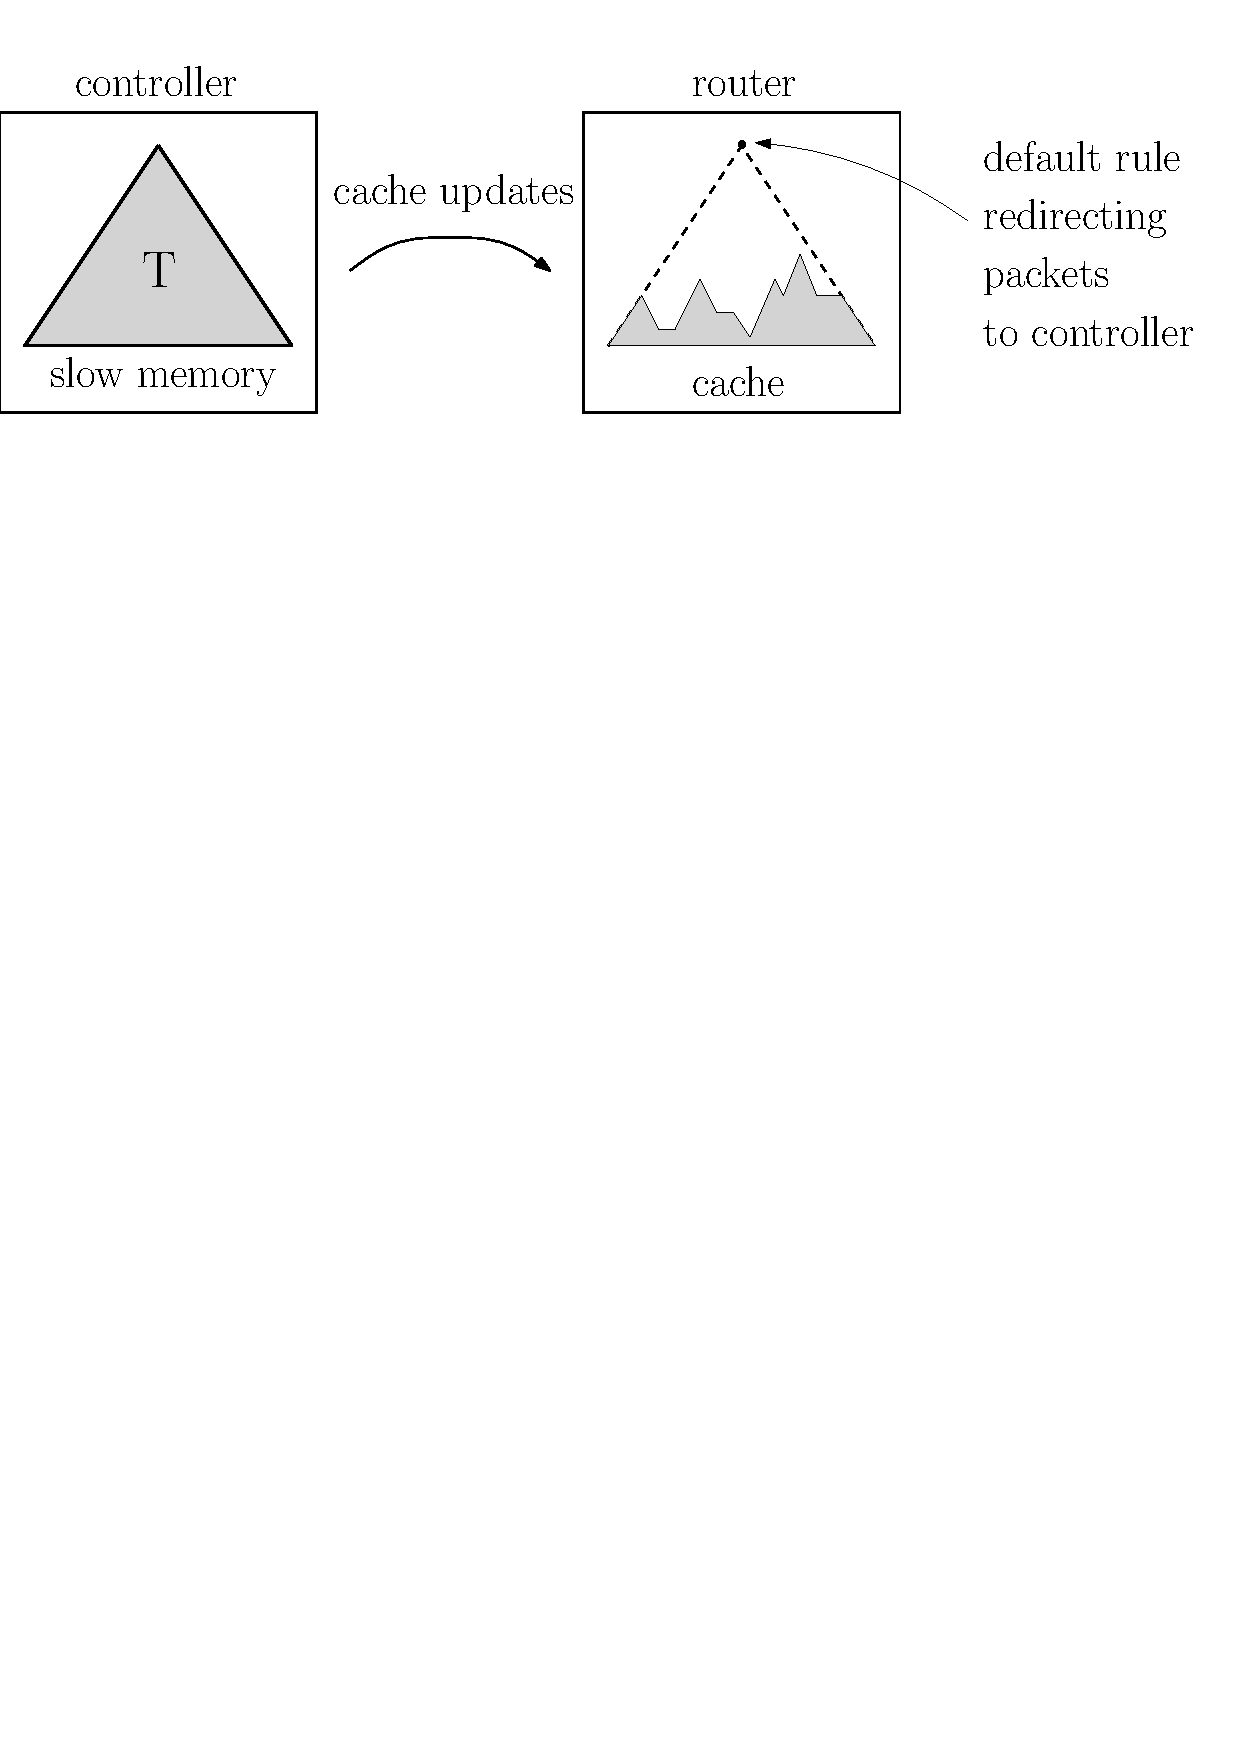
\includegraphics[width=0.7\columnwidth]{figs/cache-management/router.pdf}
\caption{The router (\emph{right}) caches only a subset of all rules, and
  rules that are not cached are answered by the controller (\emph{left}) that
  keeps the whole tree of rules. Updates to the rules are passed by the
  controller to the router.}\label{fig:router}
\end{figure}




Upon the forwarding table cache miss, the control plane may decide to update the cached portion of the forwarding table kept in the forwarding component.
Standard caching-related problems arise, such as: which entry to evict to provide space to store the new one.
Immediate update might seem a rational strategy, but in scenarios with highly dynamic networks that rearrange often, it might be beneficial to delay the update.
Premature update might result in the situation, where more time is spent alternating the cache configuration than processing packets (this is similar to \emph{thrashing} in virtual memory systems).

In the traditional caching problem, the cache elements are independent: it is always feasible to pull in or out the elements of the cache regardless of cache configuration.

\todo{todo}


Dependencies among to-be-cached items arise in numerous settings and are a
natural refinement of many caching problems. To give a concrete example, one
important application for our tree-based dependency model arises in the context
of IP routers. In particular, the online tree caching problem we introduce in
this paper is motivated by router memory constraints in IP-based networks. The
material presented in this section serves for motivation, and is not necessary
for understanding the remainder of the paper.

Nowadays, routers have to store an~enormous number of forwarding rules: the
number of rules has doubled in the last six years~\cite{bgp-routeviews} and
the superlinear growth is likely to be sustained~\cite{steve-myth}. This
entails large costs for Internet Service Providers: fast router memory
(usually Ternary Content Addressable Memory (TCAM)) is expensive and
power-hungry~\cite{tcam-expensive}.  Many routers currently either operate at
(or beyond) the edge of their memory capacities. A~solution, which could delay
the need for expensive or impossible memory upgrades in routers, is to store
only a subset of rules in the actual router and store all rules on a~secondary
device (for example a commodity server with a large but slow
memory)~\cite{cacheflow,route-caching-flat,prefix-caching,fib-caching-non-overlapping,fibium-zipf}.

This solution is particularly attractive with the advent of Soft\-ware-Defined
Network (SDN) technology, which allows to manage the expensive memory using a
software controller~\cite{cacheflow,fibium-zipf}. In particular, our
theoretical model can describe real-world architectures
like~\cite{cacheflow,fibium-zipf},
that is, our model formalizes the underlying operational
problems of such architectures. Our 
algorithm, when applied in the context of such architectures, can 
hence be used to prolong the lifetime of IP routers.

\paragraph{Setup, positive requests, fetches and evictions.}

The setup (see~\cite{fibium-zipf} for a more technical discussion) depicted in
\lref[Figure]{fig:router} consists of two entities: the actual router 
(e.g., an OpenFlow switch) which caches only a~subset of all forwarding rules,
and the (SDN) controller, which keeps all rules in its less expensive and
slower memory. During runtime, packets arrive at the router, and if an
appropriate forwarding rule is found within the rules cached by the router,
then the packet is forwarded accordingly, and the associated cost is zero.
Otherwise, the packet has to be forwarded to the controller (where 
an~appropriate forwarding rule exists); this indirection costs~$1$. Hence, the
rules correspond to cacheable items and accesses to rules are modeled by
positive requests to the corresponding items. At some chosen points in time,
the caching algorithm run at the controller may decide to remove or add rules
to the cache. Any such change entails a~fixed cost $\alpha$.\footnote{This
cost corresponds to the transmission of a message from the controller to the
router as well as the update of internal data structures of the router. Such
an update of proprietary and vendor-dependent structures can be quite
costly~\cite{tcam-expensive-updates}, but the empirical studies show it to be
independent of the rule being updated~\cite{fib-updates}.}


\paragraph{Negative requests.}

Additionally, a rule may need to be updated. For example, due to a~change
communicated by a dynamic routing protocol (e.g., BGP) the action defined by
a~rule has to be modified. In either case, we have to update the rules at the
controller: we assume that this cost is zero. (This cost is unavoidable for
any algorithm, so such an assumption makes our problem only more difficult.)
Furthermore, if the rule is also stored at the router, then we have to pay a~fixed
cost of $\alpha$ for updating the router (see the remark for the cost of
fetches and evictions). Such penalties can be easily simulated in our model:
we issue a~sequence of $\alpha$ negative requests to the updated node.  It is
straightforward to show that the costs in these two models can differ by a
factor of at most $2$. For a~formal argument, see
\lref[Appendix]{sec:bisimulation}.

\paragraph{Implementability.}

Note that the whole input (fed to a tree caching algorithm) is created at the
controller: positive requests are caused by cache misses (which redirect
packet to the controller) and batches of $\alpha$ negative requests are caused
by updates sent to the dynamic routing algorithm run at the controller.
Therefore, the whole tree caching algorithm can be implemented in software
in the controller only. Furthermore, our algorithm is a simple counter-based
scheme, which can be implemented efficiently and also fine-tuned for speed,
see \lref[Section]{sec:implementing_counters}.



\section{Problem Definition}\label{sec:preliminaries}

%In the classic online paging problem, items of some universe are requested by
%a~processing entity (e.g., blocks of RAM are requested by the processor). To
%speed up the access, computers use a faster memory, called
%\emph{cache}, capable of accommodating $k$ such items. Upon a~request to a
%non-cached item, the algorithm has to fetch it into the cache, paying a fixed
%cost, while a request to a cached item is free. If the cache is full, the
%algorithm has to free some space by evicting an arbitrary subset of items from
%the cache.
%
%The paging problem is inherently online: the algorithm has to make decisions
%what to evict from the cache without the knowledge of future requests; its
%cost is compared to the cost of an optimal \emph{offline} solution and the
%worst-case ratio of these two amounts is called \emph{competitive ratio}. The first
%analysis of this basic problem in an online model was given over three
%decades ago by Sleator and Tarjan~\cite{competitive-analysis}. The problem was later
%considered in a~variety of flavors. In particular, some papers considered a
%\emph{bypassing model}~\cite{caching-rejection-penalties,paging-irani}, where
%item fetching is optional: the requested item can be served without being in
%the cache, for another fixed cost (usually being at most the cost of item
%fetching).

In this chapter, we introduce a natural extension of an online paging problem, where
items have inter-de\-pen\-den\-cies.
In the classic online paging problem, items of some universe are requested by
a~processing entity (e.g., blocks of RAM are requested by the processor). To
speed up the access, computers use a faster memory, called
\emph{cache}, capable of accommodating $k$ such items. Upon a~request to a
non-cached item, the algorithm has to fetch it into the cache, paying a fixed
cost, while a request to a cached item is free. If the cache is full, the
algorithm has to free some space by evicting an arbitrary subset of items from
the cache.
The model variant, where fetching is optional (the requested item can be served without being in the cache, incurring some fixed cost) is called a \emph{bypassing model}.


In our model, we assume that the universe is
an arbitrary (not necessarily binary) rooted tree $T$ and the requested items
are its nodes. For any tree node $v$, $T(v) \subseteq T$ is a subtree rooted
at $v$ containing $v$ and all its descendants. We require the following
property: if a~node $v$ is in the cache, then all nodes of $T(v)$ are also
cached. In other words, we require that \emph{the cache is a~subforest of
$T$}, i.e., a union of disjoint subtrees of~$T$.  We call this problem
\emph{online tree caching}.

We assume discrete time slotted into rounds, with round $t \geq 1$
corresponding to time interval $(t-1,t)$. In round $t$, the algorithm is given
one (positive or negative) request to exactly one tree node and has to process
it, i.e., pay associated costs (if any). 
Furthermore, we assume a bypassing model and distinguish between two types of
requests: a~request can be either \emph{positive} or \emph{negative}. The
positive requests correspond to ``normal'' requests known from caching
problems: we pay~$1$ if the node is not cached; for a negative request, we pay
$1$ if the corresponding request is cached.

After serving the request, we may
reorganize our cache arbitrarily, but the resulting cache has to still be a
subforest of $T$. We pay $\alpha$ for fetching or evicting any single node,
where $\alpha \geq 1$ is an integer and a~parameter of the problem. Our goal
is to minimize the overall cost of maintaining the cache and serving the
requests.

Right after round~$t$, at time $t$,
the algorithm may arbitrarily reorganize its cache, (i) ensuring that the
resulting cache is a subforest of $T$ (i.e., if the cache contains node $v$,
then it contains the entire~$T(v)$) and (ii)~preserving the cache capacity
constraint. An algorithm pays $\alpha$ for a~single node fetch or eviction. We
denote the contents of the cache at round $t$ by $C_t$. (As the cache changes
contents only between rounds, $C_t$ is well defined.) We assume that $\alpha$
is an even integer (this assumption may change costs at most by a constant
factor). We assume that the algorithm starts with the empty cache.
%%%%%%%%%%%%%%%%%%%%%%%%%%%%%%%%%%%%%%%%%%%%%%%%%%%%%%%%%%%%%%%%%%%%%%%%%%%%%%%%%%%
%%%%%%%%%%%%%%%%%%%%%%%%%%%%%%%%%%%%%%%%%%%%%%%%%%%%%%%%%%%%%%%%%%%%%%%%%%%%%%%%%%%

\section{Algorithm}\label{sec:algo}

The algorithm \textsc{Tree Caching} (\ALGTC) presented in the following is
a simple scheme that follows a \emph{rent-or-buy paradigm}: it fetches (or evicts)
a changeset $X$ if the cost associated with requests at $X$ reaches the cost of 
such fetch or eviction.
More concretely, \ALGTC operates in multiple phases. The first phase starts at time $0$.
\ALGTC starts each phase with the empty cache and proceeds as follows. Within a
phase, every node keeps a~counter, which is initially zero. If at round~$t$ it
pays~$1$ for serving the request, it increments its counter. Whenever a node
is fetched or evicted from the cache, its counter is reset to zero. Note that
this implies that the counter of $v$ is equal to the number of negative
(positive) requests to $v$ since its last fetching to the cache (eviction from
the cache). For a~set $A \subseteq T$, we denote the sum of all counters in
$A$ at time $t$ by $\cnt_t(A)$.

We call a non-empty set $X$ a \emph{valid positive changeset} for cache $C$ if
$X \cap C = \emptyset$ and $C \cup X$ is a subforest of~$T$, and a~\emph{valid
negative changeset} if $X \subseteq C$ and $C \setminus X$ is a subforest of
$T$. We call $X$ a~\emph{valid changeset} if it is either valid positive or
negative changeset. Note that the union of positive (negative) changesets is
also a valid positive (negative) changeset. We say that the algorithm applies
changeset~$X$, if it fetches all nodes from~$X$ (for a positive changeset) and
evicts all nodes from $X$ (for a negative one). Note that not all valid
changesets may be applied as the algorithm is also limited by its cache capacity
($\kALG$ for an online algorithm and $\kOPT$ for the optimal offline one).


At time~$t$, \ALGTC verifies whether
there exists a~valid changeset $X$, such that
\begin{itemize}
\item \emph{(saturation property)} $\cnt_t(X) \geq |X| \cdot \alpha$ and
\item \emph{(maximality property)} $\cnt_t(Y) < |Y| \cdot \alpha$ for any valid
  changeset $Y \supsetneq X$.
\end{itemize}
In this case, the algorithm modifies its cache applying~$X$. 
If, at time $t$, \ALGTC is supposed to fetch some set $X$, but by doing so it
would exceed the cache capacity $\kALG$, it evicts all nodes from the cache
instead, and starts a~new phase at time~$t$. Such a \emph{final eviction}
might not be present in the last phase, in which case we call it
\emph{unfinished}. 


In \lref[Lemma]{lem:no_over-requested_changesets} (below), we show that at any
time, all valid changesets satisfying both properties of \ALGTC are either all
positive or all negative. Furthermore, right after the algorithm applies a
changeset, no valid changeset satisfies saturation property.

%%%%%%%%%%%%%%%%%%%%%%%%%%%%%%%%%%%%%%%%%%%%%%%%%%%%%%%%%%%%%%%%%%%%%%%%%%%%%%%%%%%
%%%%%%%%%%%%%%%%%%%%%%%%%%%%%%%%%%%%%%%%%%%%%%%%%%%%%%%%%%%%%%%%%%%%%%%%%%%%%%%%%%%


\section{Analysis of TC}
\label{sec:analysis}

We denote the height of $T$ by $h(T)$.  A
\emph{tree cap} rooted at $v$ is ``an~upper part'' of $T(v)$, i.e., it
contains $v$ and if it contains node~$u$, then it also contains all nodes on
the path from $u$ to $v$. If $A \subseteq B$ are both tree caps rooted at $v$,
then we say that $A$ is a tree cap of $B$.


Throughout this chapter, we fix an input $I$, its partition into phases, and
analyze both \ALGTC and \OPT on a~single fixed phase $P$. We denote the times at
which $P$ starts and ends by $\beP$ and $\enP$, respectively, i.e., rounds in
$P$ are numbered from $\beP+1$ to $\enP$. A proof of the following technical
lemma follows by induction and is presented in 
\lref{sec:proof_of_lemma_1}.


\begin{lemma}
\label{lem:no_over-requested_changesets}
Fix any time $t > \beP$. For any valid changeset $X$ for $C_t$, it holds that
$\cnt_t(X) \leq |X| \cdot \alpha$. If a~changeset $X$ is applied at time $t$,
the following properties hold:
\begin{enumerate}
\item $X$ contains the node requested at round $t$, 
\label{lemit:1}
\item $\cnt_t(X) = |X| \cdot \alpha$, 
\label{lemit:2}
\item $\cnt_t(Y) < |Y| \cdot \alpha$ for any valid changeset $Y$ for~$C_{t+1}$
(note that $C_{t+1}$ is the cache state right after application of $X$),
\label{lemit:3}
\item $X$ is a tree cap of a tree from $C_{t+1}$ if
$X$ is positive and it is a~tree cap of a tree from $C_t$ if $X$ is
negative.
\label{lemit:4}
\end{enumerate}
\end{lemma}

In the following, we assume that no positive requests are given to nodes
inside cache and no negative ones to nodes outside of it. (This does not
change the behavior of \ALGTC and can only decrease the cost of \OPT.)

For the sake of analysis, we assume that at time $\enP$, \ALGTC actually
performs a cache fetch (exceeding the cache size limit) and then, at the same
time instant, empties the cache. This replacement only increases the cost of
\ALGTC. Let $k_P$ denote the number of nodes in the cache of $\ALGTC$ at $\enP$.
In a finished phase, we measure it after the artificial fetch, but right
before the final eviction, and thus $k_P \geq \kALG + 1$; in an unfinished
phase $k_P \leq \kALG$.

The crucial part of our analysis that culminates in
\lref[Section]{sec:shifting} is the technique of shifting requests. Namely, we
modify the input sequence by shifting requests up or down the tree, so that
the resulting input sequence (i) is not harder for \OPT and (ii) is more
structured: we may lower bound the cost of \OPT on each node separately and
relate it to the cost of \ALGTC.


%%%%%%%%%%%%%%%%%%%%%%%%%%%%%%%%%%%%%%%%%%%%%%%%%%%%%%%%%%%%%%%%%%%%%%%%%%%%%%%%%%%
%%%%%%%%%%%%%%%%%%%%%%%%%%%%%%%%%%%%%%%%%%%%%%%%%%%%%%%%%%%%%%%%%%%%%%%%%%%%%%%%%%%

\subsection{Event Space and Fields}
\label{sec:event}

In our analysis, we look at a two-dimensional, discrete, spatial-temporal
space, called the \emph{event space}. The first dimension is indexed by tree
nodes, whose order is an~arbitrary extension of the partial order given by the
tree. That is, the parent of a node $v$ is always ``above''~$v$. The second
dimension is indexed by round numbers of phase~$P$. The space elements are
called \emph{slots}. Some slots are occupied by requests: a~request at node
$v$ given at round $t$ occupies slot $(v,t)$. From now on, we will identify
$P$ with a set of requests occupying some slots in the event space.

We partition slots of the whole event space into disjoint parts, called
\emph{fields}, and we show how this partition is related to the costs of \ALGTC
and \OPT. For any node~$v$ and time $t$, $\last_v(t)$ denotes the last time
strictly before~$t$, when node $v$ changed state from cached to non-cached or
vice versa; $\last_v(t) = \beP$ if $v$ did not change its state before $t$ in
phase $P$. For a~changeset~$X_t$ applied by
\ALGTC at time $t$, we define the field $F^t$ as
\[
  F^t = \left\{\ (v,r) : v \in X_t \, \wedge\, \last_v(t)+1 \leq r \leq t\ \right\}.
\]
That is, field $F^t$ contains all the requests that eventually trigger the
application of $X_t$ at time $t$. We say that $F^t$ ends at $t$. We call field
$F^t$ \emph{positive} (\emph{negative}) if $X_t$ is a positive (negative)
changeset. An~example of a~partitioning into fields is given in
\lref[Figure]{fig:fields}. We define $\req(F^t)$ as the number of requests
belonging to slots of~$F^t$ and let $\sizetc(F^t)$ be the number of involved
nodes (note that $\sizetc(F^t) = |X_t|)$. The observation below follows
immediately by \lref[Lemma]{lem:no_over-requested_changesets}.

\begin{figure}[t]
  \centering
  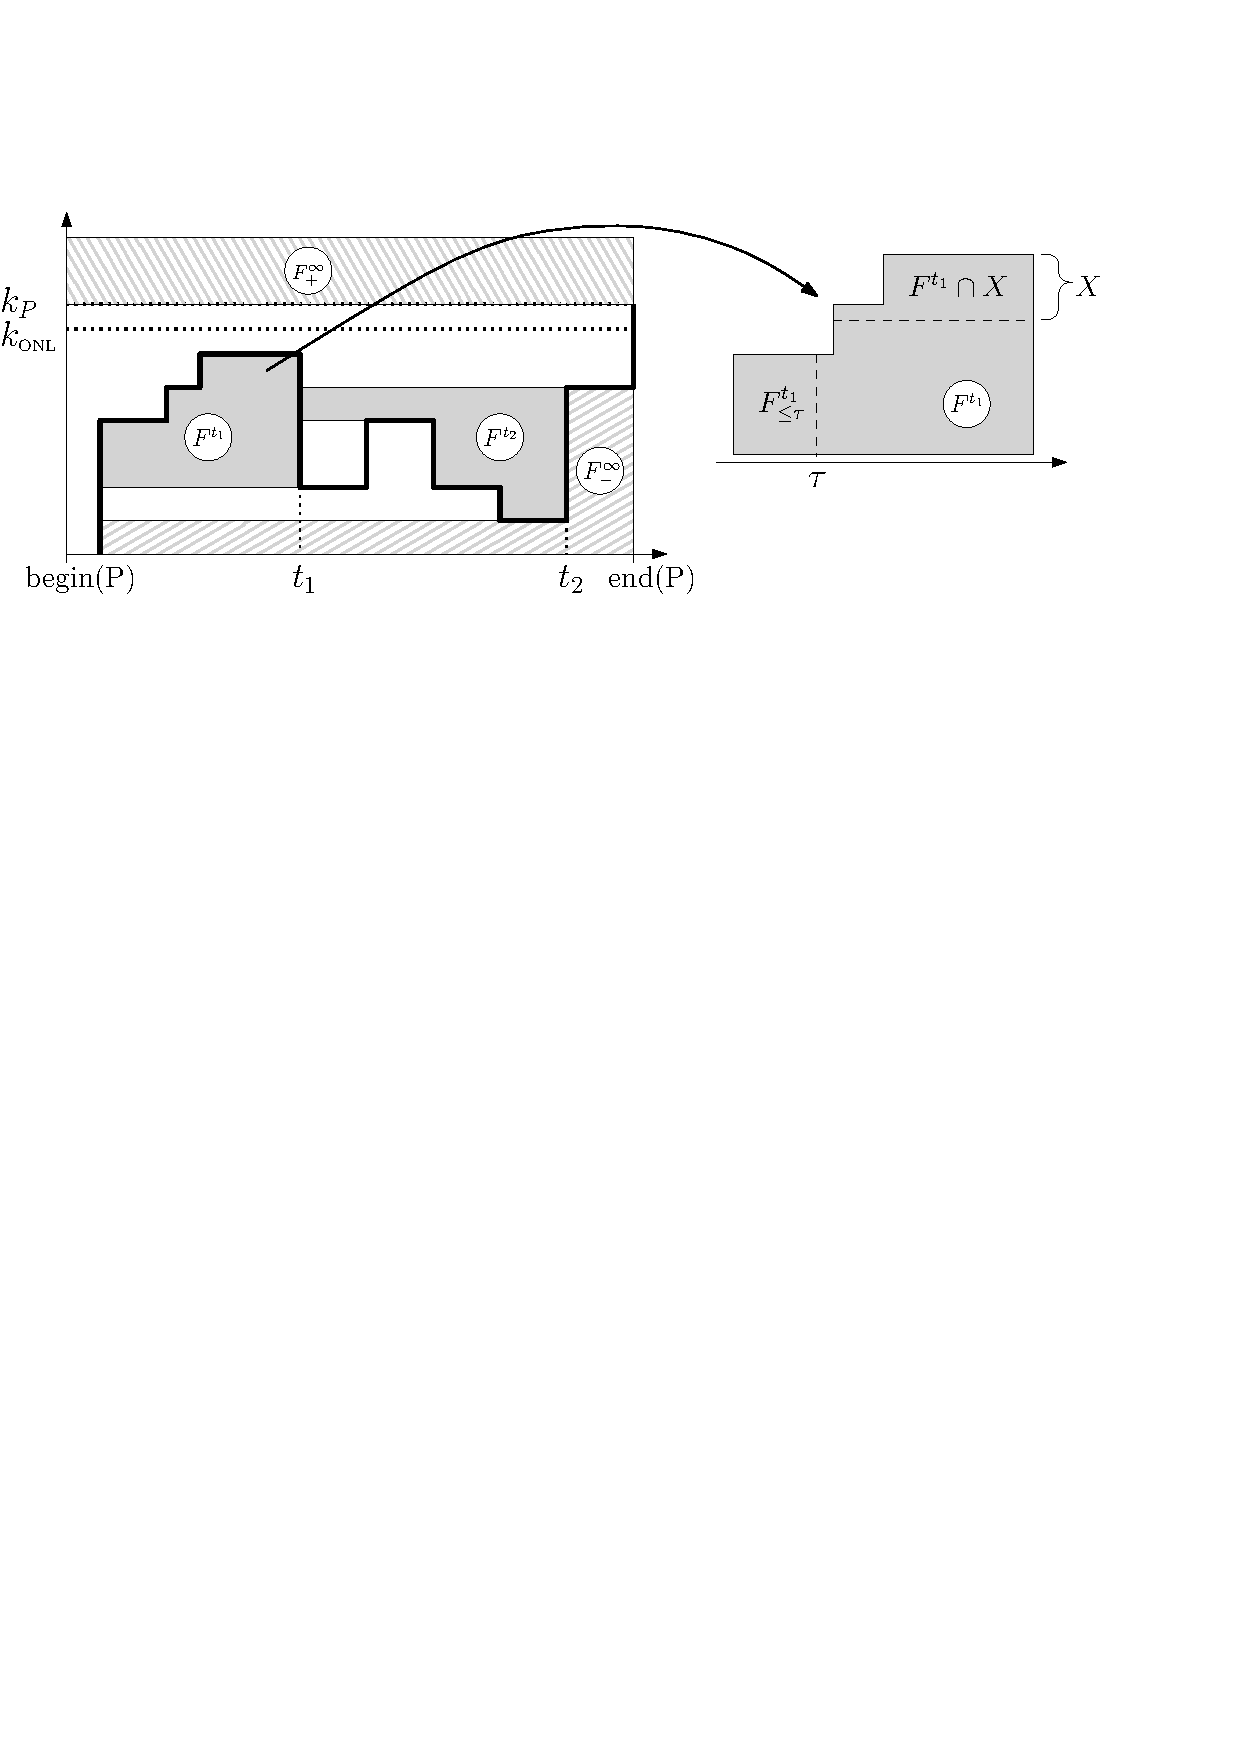
\includegraphics[width=0.99\columnwidth,keepaspectratio]{figs/cache-management/fields_horizontal}
  \caption{Partitioning of a single phase into fields for a line (a tree with
  no branches). The thick line represents cache contents. Possible final eviction
  at $\enP$ is not depicted. $F^{t_1}$ is a~negative field and $F^{t_2}$ is a
  positive one. In the particular depicted example, nodes are ordered from the
  leaf (bottom) to the root (top  of the picture). We emphasize that for a
  general, branched tree, some notions (in particular fields) no longer have
  nice geometric interpretations.}
  \label{fig:fields}
\end{figure}


\begin{observation}
\label{obs:field_requests}
For any field $F$, $\req(F) = \sizetc(F) \cdot \alpha$. All these requests are
positive (negative) if $F$ is positive (negative).
\end{observation}

Finally, we call the rest of the event space defined by phase $P$
\emph{open field} and denote it by $F^\infty$. The set of all fields except $
F^\infty$ is denoted by $\F$. Let $\sizetc(\F) = \sum_{F \in \F} \sizetc(F)$.

\begin{lemma}
\label{lem:alg_cost}
For any phase $P$ partitioned into a set of fields $\F \cup \{ F^\infty \}$,
it holds that $\ALGTC(P) \leq 2 \alpha \cdot \sizetc(\F) + \req(F^\infty) + k_P
\cdot \alpha$.
\end{lemma}

\begin{proof}
By \lref[Observation]{obs:field_requests}, the cost associated with serving
the requests from all fields from $\mathcal{F}$ is $\sum_{F \in \F} \alpha
\cdot \sizetc(F) = \alpha \cdot \sizetc(\F)$. The cost of the cache reorganization
at the fields' ends is exactly the same. The term $\req(F^\infty)$ represents
the cost of serving the requests from $F^\infty$ and $k_P \cdot \alpha$
upper-bounds the cost of the final eviction (not present in an unfinished
phase).
\end{proof}



%%%%%%%%%%%%%%%%%%%%%%%%%%%%%%%%%%%%%%%%%%%%%%%%%%%%%%%%%%%%%%%%%%%%%%%%%%%%%%%%%%%
%%%%%%%%%%%%%%%%%%%%%%%%%%%%%%%%%%%%%%%%%%%%%%%%%%%%%%%%%%%%%%%%%%%%%%%%%%%%%%%%%%%

\subsection{Shifting Requests}\label{sec:shifting}

The actual challenge in the proof is to relate the structure of the fields to
the cost of {\OPT}. The rationale behind our construction is based on the
following thought experiment. Assume that the phase is unfinished (for
example, when the cache is so large that the whole input corresponds to a
single phase). Recall that the number of requests in each field $F \in \F$ is
equal to $\sizetc(F) \cdot \alpha$. Assume that these requests are evenly
distributed among the nodes of $F$ (each node from $F$ receives $\alpha$
requests in the slots of $F$). Then, the history of any node $v$ is
alternating between periods spent in positive fields and periods spent in
negative fields. By our even distribution assumption, each such a period
contains exactly $\alpha$ requests. Hence, for any two consecutive periods of
a~single node, \OPT has to pay at least $\alpha$ (either $\alpha$ for positive
requests or $\alpha$ for negative ones, or $\alpha$ for changing the
cached/non-cached state of $v$). Essentially, this shows that $\OPT$ has to
pay an amount that can be easily related to $\alpha \cdot
\sizetc(\F)$.

Unfortunately, the requests may not be evenly distributed among the nodes. To
alleviate this problem, we will modify the requests in phase $P$, so that the
newly created phase $P'$ is not harder for $\OPT$ and will ``almost'' have the
even distribution property. In this construction, the time frame of $P$ and
its fields are fixed.

\subsubsection{Legal Shifts}

We say that a request placed originally (in phase $P$) at slot $(v,t)$ is
\emph{legally shifted} if its new slot is $(m(v), t)$, where (i) for a
positive request, $m(v)$ is either equal to~$v$ or is one of its descendants
and (ii) for a negative request, $m(v)$ is either equal to $v$ or is one of
its ancestors. For any fixed sequence of fetches and evictions within phase
$P$, the associated cost may only decrease when these actions are replayed on
the modified requests.

\begin{observation}
\label{obs:pprim_easier_than_p}
If $P'$ is created from $P$ by legally shifting the requests, then $\OPT(P')
\leq \OPT(P)$.
\end{observation}

The main difficulty is however in keeping the legally shifted requests within
the field they originally belonged to. For example, a negative request from
$F$ shifted at round $t$ from node~$u$ to its parent may fall out of $F$ as
the parent may still be outside the cache at round~$t$. In effect, a careless
shifting of requests may lead to a situation where, for a single node~$v$,
requests do not create interleaved periods of positive and negative requests,
and hence we cannot argue that $\OPT(P')$ is sufficiently large.

In the following subsections, we show that it is possible to legally shift the
requests of any field $F \in \F$ (i.e., shift positive requests down and negative
requests up), so that they remain within $F$, and they will
be either exactly or approximately evenly distributed among nodes of $F$.
This will create $P'$ with appropriately large cost for \OPT.

%%%%%%%%%%%%%%%%%%%%%%%%%%%%%%%%%%%%%%%%%%%%%%%%%%%%%%%%%%%%%%%%%%%%%%%%%%%%%%%%%%%
%%%%%%%%%%%%%%%%%%%%%%%%%%%%%%%%%%%%%%%%%%%%%%%%%%%%%%%%%%%%%%%%%%%%%%%%%%%%%%%%%%%

\subsubsection{Notation}
%
We start with some general definitions and remarks. For any field $F$ and set
of nodes~$A$, let $F \cap A = \{ (v,t) \in F : v \in A \}$. Analogously, if
$L$ is a set of rounds, then let $F \cap L = \{ (v,t) \in F : t \in L \}$. For
any field $F^t$ and time $\tau$, we define
\[
    F^t_{\leq \tau} = F^t \cap \left\{ t' : t' \leq \tau \right\}.
\]
It is convenient to think that $F^t$ evolves with time and $F^t_{\leq \tau}$
is the snapshot of $F^t$ at time~$\tau$. Note that $F^t$ may have some nodes
not included in $F^t_{\leq \tau}$. These objects are depicted in
\lref[Figure]{fig:fields}.

We may extend the notions of $\req$ and $\sizetc$ to arbitrary subsets of fields
in a natural way.
For any subset $S \subseteq F$, we call it \emph{over-requested} if
$\req(S) > \sizetc(S) \cdot \alpha$. 

\begin{lemma}
\label{lem:not_over-requested}
Fix any field $F^t$, the corresponding changeset $X_t$, and any time $\tau$.
\begin{enumerate}
\item If $F^t$ is negative, then for any tree cap $D$ of $X_t$, the set
    $F^t_{\leq \tau} \cap D$ is not over-requested.
\item If $F^t$ is positive, then for any subtree $T' \subseteq T$, the set
    $F^t_{\leq \tau} \cap T'$ is not over-requested.
\end{enumerate}
\end{lemma}

\begin{proof} 
As the nodes from $F^t_{\leq \tau} \cap D$ form a valid changeset at time~$\tau$, 
\lref[Lemma]{lem:no_over-requested_changesets} implies $\req(F^t_{\leq
\tau} \cap D) = \cnt_\tau(F^t_{\leq \tau} \cap D) \leq |F^t_{\leq \tau} \cap
D| \cdot \alpha$.

The proof of the second property is identical: As $F^t_{\leq \tau} \cap T'$ is
also a valid changeset at time $\tau$, by
\lref[Lemma]{lem:no_over-requested_changesets}, $\req(F^t_{\leq \tau}
\cap T') = \cnt_\tau(F^t_{\leq \tau} \cap T')
\leq |F^t_{\leq \tau} \cap T'| \cdot \alpha$. 
\end{proof}

By \lref[Lemma]{lem:not_over-requested} applied at $\tau = t$ and
\lref[Observation]{obs:field_requests}, we deduct the following corollary.

\begin{corollary}
\label{cor:density}
Fix any field $F^t$, the corresponding changeset $X_t$ and any tree
cap $D$ of $X_t$. 
\begin{enumerate}
\item If $F^t$ is positive, then $\req(F^t \cap D) \geq \alpha \cdot |D|$.
\item If $F^t$ is negative, then $\req(F^t \cap (X_t \setminus D)) \geq 
  \alpha \cdot \text{$|X_t \setminus D|$}$.
\end{enumerate}
\end{corollary} 

Informally speaking, the corollary above states that the average amount of
requests in a~positive field is \emph{at least as large at the top of the
field as at its bottom}. For a negative field this relation is reversed.


%%%%%%%%%%%%%%%%%%%%%%%%%%%%%%%%%%%%%%%%%%%%%%%%%%%%%%%%%%%%%%%%%%%%%%%%%%%%%%%%%%%
%%%%%%%%%%%%%%%%%%%%%%%%%%%%%%%%%%%%%%%%%%%%%%%%%%%%%%%%%%%%%%%%%%%%%%%%%%%%%%%%%%% 



\subsubsection{Shifting Negative Requests Up}
\label{sec:negative_shifting}
  
Fix a valid negative changeset $X_t$ applied at time~$t$ and the
corresponding field~$F^t$. We call a~tree cap \mbox{$Y \subseteq X_t$} \emph{proper} if
\begin{enumerate}
\item $\req(F^t \cap Y) = |Y| \cdot \alpha$ and
\item $F^t_{\leq \tau} \cap D$ is not over-requested for any tree cap $D \subseteq Y$ and any time 
$\tau \leq t$.
\end{enumerate}

The first property of \lref[Lemma]{lem:not_over-requested} states that before
we shift the requests of $F_t$, the set $X_t$ is proper.  We start with $Y =
X_t$, and proceed in a bottom-up fashion, inductively using the lemma below.
We take care of a~single node of $Y$ at a time and ensure that after the shift
the number of requests at this node is exactly $\alpha$ and the remaining part
of $Y$ remains proper.

\begin{lemma}
\label{lem:shift_up_and_stay_proper}
Given a negative field $F^t$, the corresponding changeset~$X_t$ and 
a proper tree cap $Y \subseteq X_t$, it is possible to choose a leaf $v$ 
and legally shift some requests inside $Y$,
so that in result $\req({v}) = \alpha$ and $Y \setminus \{v\}$ is proper.
\end{lemma}

\begin{proof}
As $\req(F^t \cap Y) = |Y| \cdot \alpha$, \lref[Corollary]{cor:density}
implies that any leaf of $Y$ was requested at least $\alpha$ times
inside~$F^t$. We pick an arbitrary leaf $v$, and let $r \geq \alpha$ be the
number of requests to $v$ in $F^t$.

We look at all the requests to $v$ in $F^t$ ordered by their round. Let $s$ be
the round when $(\alpha+1)$-th of them arrives. We will now show that at round
$s$, \ALGTC already has $p(v)$ in its cache. If it had not, $\{v\}$ would be a
tree cap of $F^t_{\leq s}$, and by the first property of
\lref[Lemma]{lem:not_over-requested}, it would contain at most $\alpha$
requests, which is a~contradiction. Hence, if we shift the chronologically
last $r - \alpha$ requests from $v$ to $p(v)$, these requests stay within
$F^t$.

It remains to show that $Y \setminus \{v\}$ is proper after such a shift. We
choose any tree cap $D \subseteq Y$ and any time \mbox{$\tau \leq t$}. If $D$
does not contain $p(v)$ or $\tau < s$, then the number of requests in
$F^t_{\leq \tau} \cap D$ was not changed by the shift, and hence $F^t_{\leq
\tau} \cap D$ is not over-requested. Otherwise, $D \cup \{v\}$ was a tree cap
in $Y$ and by the lemma assumption, $F^t_{\leq \tau} \cap (D \cup \{v\})$ was
not over-requested. As $F^t_{\leq \tau} \cap D$ has now exactly $\alpha$ less
requests than $F^t_{\leq \tau} \cap (D \cup \{v\})$ had, it is not
over-requested, either.
\end{proof}

\begin{corollary}
\label{cor:crucial_lemma_neg}
For any negative field $F^t$, it is possible to legally shift its requests up,
so that they remain within $F^t$ and after the modification each node is
requested exactly $\alpha$ times.
\end{corollary}


%%%%%%%%%%%%%%%%%%%%%%%%%%%%%%%%%%%%%%%%%%%%%%%%%%%%%%%%%%%%%%%%%%%%%%%%%%%%%%%%%%%
%%%%%%%%%%%%%%%%%%%%%%%%%%%%%%%%%%%%%%%%%%%%%%%%%%%%%%%%%%%%%%%%%%%%%%%%%%%%%%%%%%%

\subsubsection{Shifting Positive Requests Down}
\label{sec:positive_shifting}

We will now focus on the problem of shifting the positive requests down in a
single positive field $F^t$, corresponding to a single fetch of \ALGTC at the
time $t$. Our goal is to devise a shifting strategy, that will result in at
least $\Omega(\sizetc(F^t)/h(T))$ nodes having $\alpha/2$ requests each. While
this result may be suboptimal, deriving a shifting strategy for a~positive
field that would have the same equal distribution guarantee as the one
provided by \lref[Corollary]{cor:crucial_lemma_neg} is not possible.

First, we prove that from any node $v$ in the field, we can shift down a
constant fraction of its requests within the field, distributing them to
different nodes.

\begin{lemma}
\label{lem:downshift}
Let $F^t$ be a positive field and let $X_t$ be the corresponding changeset
fetched to the cache at time~$t$. Fix any node $v \in X_t$ that has been
requested at least $c \cdot (\alpha / 2)$ times in~$F^t$, where $c$ is an
integer. It is possible to shift down its requests to the nodes of $T(v) \cap
X_t$, so that these requests remain inside $F^t$ and $\lceil c / 2 \rceil$
nodes of $T(v)$ get $\alpha / 2$ requests each.
\end{lemma}

\begin{proof}
We order the nodes $u_1, u_2, \ldots u_{|T(v) \cap X_t|}$ of $T(v) \cap X_t$,
so that $\last_{u_i}(t) \leq \last_{u_{i+1}}(t)$ for all $i$. In case of a
tie, we place nodes that are closer to $v$ first. Note that this linear
ordering is an~extension of the partial order defined by the tree: the parent
of a~node cannot be evicted later than the node itself (otherwise the cache
would cease to be a subforest of $T$). In particular, it holds that $u_1 = v$.

We number $c \cdot (\alpha / 2)$ requests to $v$ chronologically, starting
from $1$. For any $j \in \{1, \ldots, \lceil c/2 \rceil \}$ we look at round
$\tau_j$ with the $((j-1) \cdot \alpha + 1)$-th request to $v$. When this
request arrives, node $u_j$ is already present in the cache. Otherwise, we
would have at least \mbox{$j \cdot \alpha + 1$} requests in $F^t_{\leq
{\tau_j}} \cap \{u_1, \ldots, u_j\}$ (already in $F^t_{\leq {\tau_j}}
\cap \{u_1\}$ alone), which would make it over-requested, and thus contradict
the second property of \lref[Lemma]{lem:not_over-requested}. Hence, we may
take requests numbered from $(j-1) \cdot \alpha + 1$ to $(j-1) \cdot \alpha +
\alpha/2$, shift them down from $v$ to $u_j$, and after such modification
these requests are still inside $F^t$. Note that for $j = 1$ requests are not
really shifted, as $u_1$ is $v$ itself. We perform such shift for any $j \in
\{1, \ldots, \lceil c/2 \rceil \}$, which yields the lemma.
\end{proof}
  
\begin{lemma}
\label{lem:crucial_lemma_pos}
For any positive field $F^t$, it is possible to legally shift its requests
down, so that they remain within $F^t$ and after the modification at least
$\sizetc(F^t)/(2 h(T))$ nodes in $F^t$ have at least $\alpha/2$ requests each.
\end{lemma}

\begin{proof}
Let $X_t$ be the changeset corresponding to field $F^t$, which is fetched to the cache
at time~$t$. By \lref[Observation]{obs:field_requests}, $\req(F^t) = |X_t|
\cdot \alpha$. We gather the requests at every node into groups of $\alpha/2$
consecutive requests. In every node at most $\alpha/2$ requests remain not
grouped. Let $\overline\req(X)$ denote the number of grouped requests in the
set $X$. Clearly, $\overline\req(F^t) \geq |X_t| \cdot \alpha / 2$, i.e.,
there are at least $|X_t|$ groups of requests in set $X_t$.

Let $X_t = X_t^1 \sqcup X_t^2 \sqcup \dots \sqcup X_t^{h(T)}$ be a partition
of the nodes of the tree $X_t$ into layers according to their distance to the
root. By the pigeonhole principle, there is a layer $X_t^i$ containing at
least $\lceil |X_t| / h(T) \rceil$ groups of requests (each group has
$\alpha/2$ requests).

Nodes of $X_t^i$ are independent, i.e., for $u, v \in X_t^i$ the trees $T(u)$
and $T(v)$ are disjoint. Therefore, we may use the shifting strategy described
in \lref[Lemma]{lem:downshift} for each node of $X_t^i$ separately. After such
modification, at least $\lceil |X_t| / (2 h(T)) \rceil \geq \sizetc(F_t) / (2
h(T))$ nodes have at least $\alpha / 2$ requests each.
\end{proof}


%%%%%%%%%%%%%%%%%%%%%%%%%%%%%%%%%%%%%%%%%%%%%%%%%%%%%%%%%%%%%%%%%%%%%%%%%%%%%%%%%%%
%%%%%%%%%%%%%%%%%%%%%%%%%%%%%%%%%%%%%%%%%%%%%%%%%%%%%%%%%%%%%%%%%%%%%%%%%%%%%%%%%%%

\subsubsection{Using Request Shifting for Bounding OPT}
\label{sec:lower-bound}

Finally, we may use our request shifting to relate $\sizetc(\F) =
\sum_{F \in \mathcal{F}} \sizetc(F)$ to the cost of $\OPT$ in a single phase $P$.
Recall that $k_P$ denotes the size of \ALGTC's cache at the end of $P$. We
assume that {\OPT} may start the phase with an arbitrary state of the cache.

\begin{lemma}
\label{lem:leftovers}
For any phase $P$, $\OPT(P) \geq (\sizetc(\F) / (4 h(T)) - k_P)
\cdot \alpha/2$.
\end{lemma}

\begin{proof}
We transform $P$ using legal shifts that are described in 
\lref[Section]{sec:negative_shifting} and
\lref[Section]{sec:positive_shifting}. That is, we create a~corresponding
phase $P'$ that satisfies both
\lref[Corollary]{cor:crucial_lemma_neg} and
\lref[Lemma]{lem:crucial_lemma_pos}. 
By \lref[Observation]{obs:pprim_easier_than_p}, it is sufficient to show that
$\OPT(P') \geq (\sizetc(\F) / (4 h(T)) - k_P) \cdot \alpha/2$.

\begin{figure}[t]
\centering
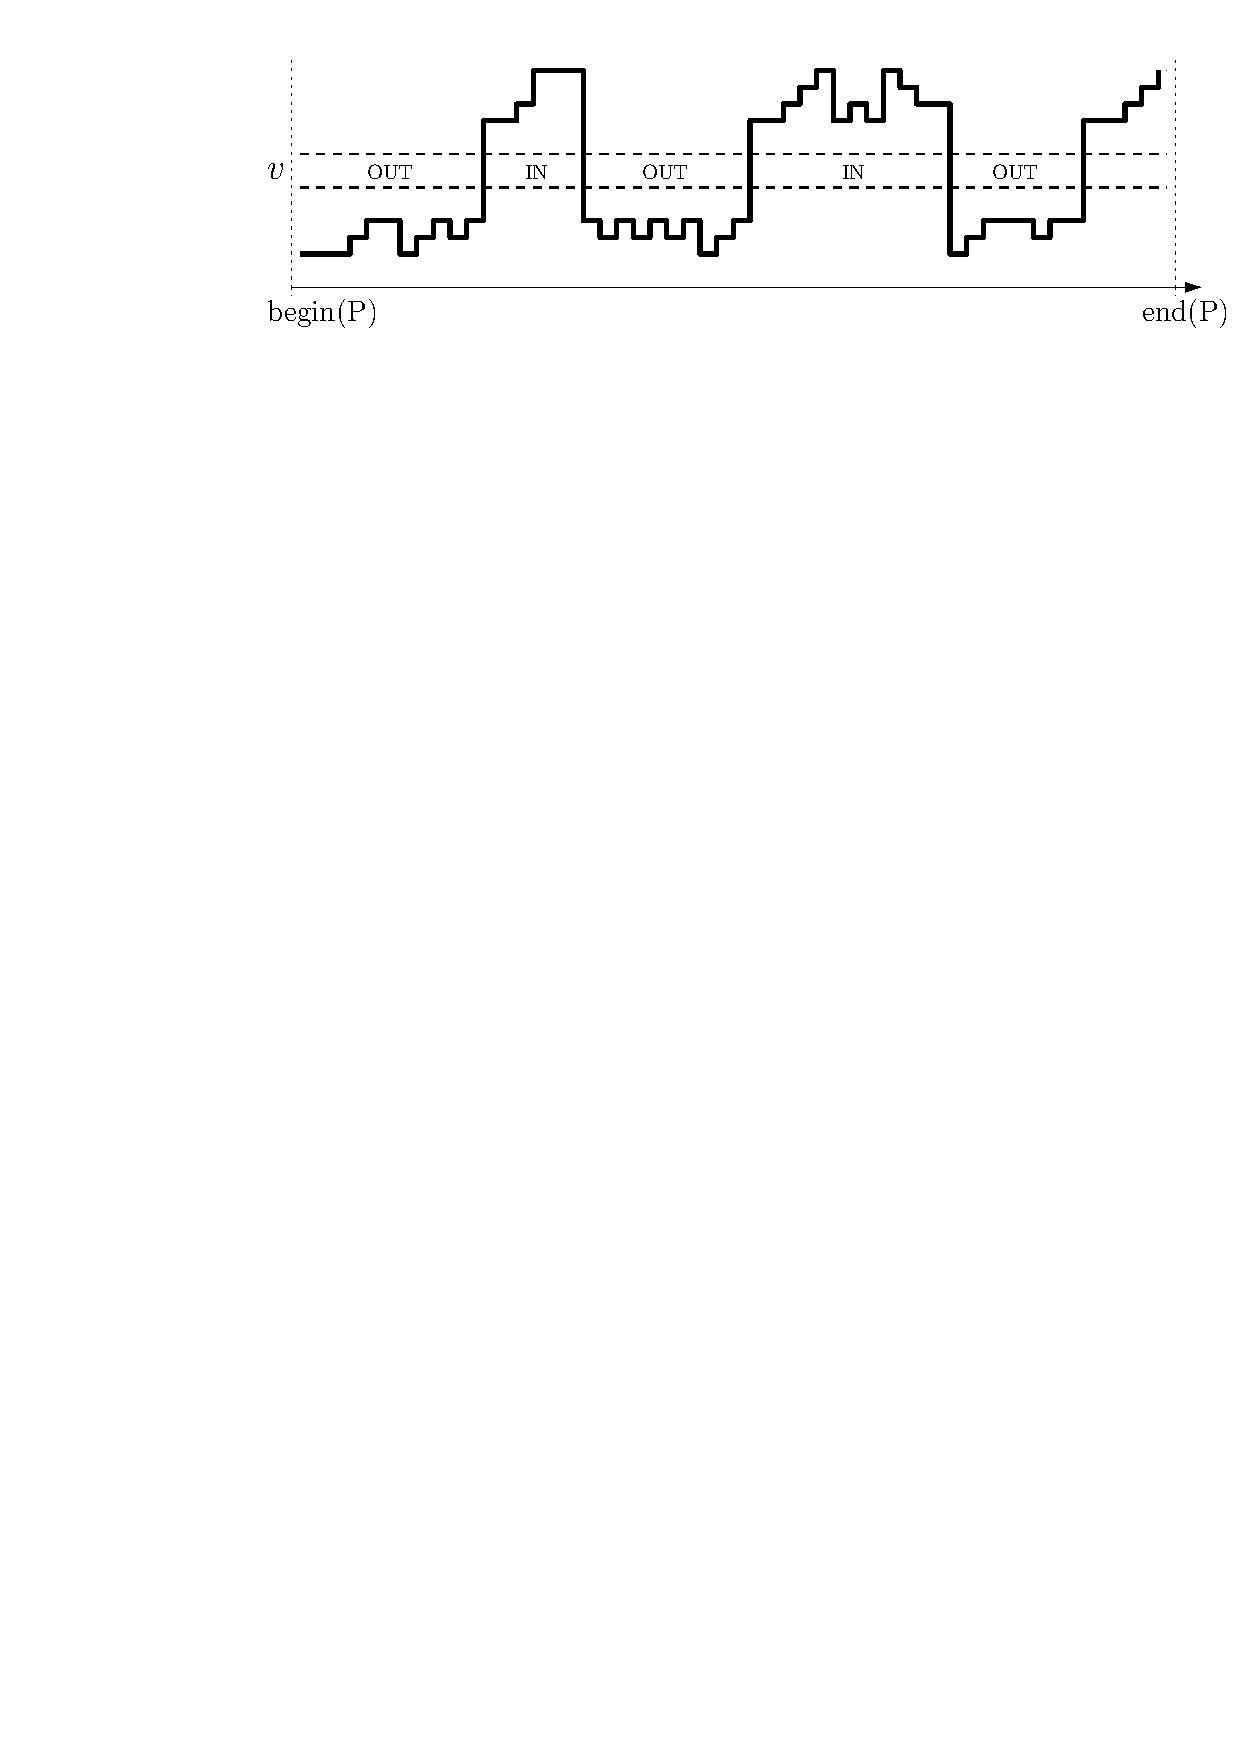
\includegraphics[width=0.9\columnwidth,keepaspectratio]{figs/cache-management/leftover}
\caption{Partitioning of the phase into interleaving \pin and \pout periods
for node $v$. The thick line represents cache contents. The \emph{leftover}
\pout period (the last one) is present for node $v$ as it has finished phase
$P$ inside \ALGTC's cache. The periods can be followed by requests contained in
$F^\infty$.}
\label{fig:leftover}
\end{figure}

We focus on a single node $v$.  We cut its history into interleaved periods:
\pout \emph{periods}, when $v$ is outside the cache and receives positive 
requests, and \pin \emph{periods} when \ALGTC keeps $v$ in the cache and $v$
receives negative requests. A final (possibly empty) part corresponding to the
time when $v$ is in the $F^\infty$ field is not accounted in \pout or \pin
periods, i.e., each \pin or \pout period corresponds to some field $F \in \F$.
Let $p^\pin$ and $p^\pout$ denote the total number of \pin and \pout periods
(respectively) for all nodes during the phase. An~example is given
in~\lref[Figure]{fig:leftover}.

Recall that \ALGTC starts each phase with an empty cache, and hence each node
starts with an \pout period. For $k_P$ nodes that are in {\ALGTC}'s cache at the
end of the phase (and only for them) their history ends with an \pout period
not followed by an \pin period. We call them \emph{leftover periods}. Thus,
$p^\pout = p^\pin + k_P$. The total number of periods ($p^\pin + p^\pout$) is
equal to the total size of all \emph{fields}, $\sizetc(\F)$, and thus $p^\pout 
\geq \sizetc(\F) / 2$.

We call a period \emph{full} if it has at least $\alpha/2$ requests. The
shifting strategies described in the previous section ensure that all
\pin periods are full and at least $1/(2 h(T))$ of all \pout periods are full.
Thus, there are at least $p^\pout/(2 h(T)) - k_P$ full non-leftover \pout
periods; each of them together with the following \pin period constitutes a
\emph{full \pout-\pin pair}.

\OPT has to pay at least $\alpha/2$ for the node in the course of the history
described by a~full \pout-\pin pair: it pays $\alpha$ either for changing the
cached/non-cached state of a node, or $\alpha/2$ for all positive requests or
$\alpha/2$ for all negative ones. Thus, $\OPT(P') \geq ( p^\pout / (2 h(T)) -
k_P ) \cdot \alpha/2 \geq ( \sizetc(\F) / (4 h(T)) - k_P ) \cdot \alpha/2$.
\end{proof}


%%%%%%%%%%%%%%%%%%%%%%%%%%%%%%%%%%%%%%%%%%%%%%%%%%%%%%%%%%%%%%%%%%%%%%%%%%%%%%%%%%%
%%%%%%%%%%%%%%%%%%%%%%%%%%%%%%%%%%%%%%%%%%%%%%%%%%%%%%%%%%%%%%%%%%%%%%%%%%%%%%%%%%%

\subsection{Competitive Ratio}
\label{sec:comp_ratio}

To relate the cost of \OPT to \ALGTC in a single phase $P$, we still need to
upper-bound $\req (F^\infty)$ and relate $k_P \cdot \alpha$ to the cost of
$\OPT$ (i.e., compare the bounds on \ALGTC and \OPT provided by
\lref[Lemma]{lem:alg_cost} and \lref[Lemma]{lem:leftovers}, respectively).

For the next two lemmas, we define $\VOPT$ as the set of all nodes that were
in \OPT cache at some time of~$P$ and let $\VOPTC = T \setminus \VOPT$. Note
that $\VOPT$ is a union of subforests (nodes present in \OPT's cache at
consecutive times), and hence a subforest itself.

\begin{lemma}
\label{lem:f_infty}
For any phase $P$, it holds that $\req (F^\infty) \leq 2 \cdot \kALG \cdot
\alpha + 2 \cdot \OPT(P)$.
\end{lemma}

\begin{proof}
We assume first that $P$ is a finished phase. Then, $P$ ends with an
artificial fetch of $X_{\enP}$ at time $\enP$ (followed by the final eviction).
We split $F^\infty$ into two disjoint parts (see \lref[Figure]{fig:fields}):
\begin{align*}
  F^\infty_- = &\; \{(v, t): v \in C_{\enP}, t \geq \last_v(\enP)\}, \\
  F^\infty_+ = &\; \{(v, t): v \notin C_{\enP} \sqcup X_{\enP}, \,
           t \geq \last_v(\enP)\}.
\end{align*}
Note that $F^\infty_-$ contains only negative requests and $F^\infty_+$ only
positive ones. As $\req(F^\infty) = \req(F^\infty_-) + \req (F^\infty_+ \cap
\VOPTC) + \req (F^\infty_+ \cap \VOPT)$, we estimate each of these summands
separately.
\begin{itemize}
\item
Nodes from $F^\infty_-$ are in the cache $C_{\enP}$ and were not
evicted from the cache. Thus, $\req(F^{\infty}_-) \leq |C_{\enP}| \cdot \alpha
\leq \kALG \cdot \alpha$.
\item
All the requests from $\VOPTC$ are paid by \OPT, and hence
$\req(F^\infty_+ \cap \VOPTC) \leq \req(\VOPTC) \leq \OPT(P)$.
\item
$F^\infty_+$ is a valid changeset for cache $C_{\enP} \sqcup X_{\enP}$.
As $\VOPT$ is a subforest of $T$, $F^\infty_+ \cap \VOPT$ is also a valid
changeset for the cache $C_{\enP} \sqcup X_{\enP}$. Therefore, $\req
(F^\infty_+ \cap \VOPT) \leq \sizetc(F^\infty_+ \cap \VOPT) \cdot \alpha$, as
otherwise the set fetched at time $\enP$ would not be maximal. (\ALGTC could
then fetch $X_{\enP} \sqcup (F^\infty_+ \cap \VOPT)$ instead of $X_{\enP}$.)
Thus, $\req (F^\infty_+ \cap \VOPT) \leq |\VOPT| \cdot \alpha = \kOPT \cdot
\alpha + (|\VOPT| - \kOPT)
\cdot \alpha \leq \kALG \cdot \alpha + \OPT(P)$.
The last inequality follows as --- independently of the initial state --- \OPT
needs to fetch at least $|\VOPT| - \kOPT$ nodes to the cache during $P$.
\end{itemize}
Hence, in total, $\req (F^\infty) \leq 2 \cdot \kALG \cdot
\alpha + 2 \cdot \OPT(P)$ for a finished phase $P$.

We note that if there was no cache change at $\enP$, the analysis above would
hold with $X_{\enP} = \emptyset$ with virtually no change. Therefore, for an
unfinished phase $P$ ending with a fetch or ending without cache change at
$\enP$, the bound on $\req(F^\infty)$ still holds. However, if an unfinished
phase~$P$ ends with an eviction, then we look at the last eviction-free 
time $\tau$ of~$P$. We now observe the evolution of field
$F^\infty$ from time~$\tau$ till $\enP$. At time $\tau$, $\req(F^\infty) \leq
2 \cdot \kALG \cdot \alpha + 2 \cdot \OPT(P)$. Furthermore, in subsequent
times, it may only decrease: at any round $F^\infty$ gets an additional
request, but on eviction $\req(F^\infty)$ decreases by $\alpha$ times
the number of evicted nodes (i.e., at least by $\alpha \geq 1$). Hence, the
value of $\req(F^\infty)$ at $\enP$ is also at most $2 \cdot \kALG \cdot
\alpha + 2 \cdot \OPT(P)$.
\end{proof}



By combining \lref[Lemma]{lem:alg_cost}, \lref[Lemma]{lem:leftovers} and 
\lref[Lemma]{lem:f_infty}, we immediately obtain the following corollary
(holding for both finished and unfinished phases).

\begin{corollary}
\label{cor:any_phase_bound}
For any phase $P$, it holds that 
$\ALGTC(P) \leq O(h(T)) \cdot \OPT(P) + O(h(T) \cdot (k_P + \kALG) \cdot \alpha)$.
\end{corollary}

Using the corollary above, its remains to bound the value of~$k_P$. This is
easy for an unfinished phase, as $k_P \leq \kALG$ there. For a~finished phase,
we provide another bound.

\begin{lemma}
\label{lem:opt_bound2}
For any finished phase $P$, it holds that
$k_P \cdot \alpha \leq \OPT(P) \cdot (\kALG + 1) / (\kALG + 1 - \kOPT)$.
\end{lemma}

\begin{proof}
First, we compute the number of positive requests in $\VOPTC$. Let $X_{t_1},
X_{t_2}, \ldots, X_{t_s}$ be all positive changesets applied by \ALGTC in~$P$.
For any~$t$, let $X'_t = X_t \setminus \VOPT$. As $X_t$ is some tree cap and
$\VOPT$ is a~subforest of $T$, $X'_t$ is a~tree cap of $X_t$. By
\lref[Corollary]{cor:density}, the number of requests to nodes of $X'_t$ in
field $F^t$ is at least $|X'_t| \cdot \alpha$. These requests for different
changesets $X_t$ are disjoint and they are all outside of $\VOPT$. Hence the
total number of positive requests outside of $\VOPT$ is at least $\sum_{i=1}^s
|X'_{t_i}| \cdot \alpha$, where $\sum_{i=1}^s |X'_{t_i}| \geq |\bigcup_{i=1}^s
X'_{t_i}| = |(\bigcup_{i=1}^s X_{t_i}) \setminus \VOPT| \geq |\bigcup_{i=1}^s
X_{t_i}| - |\VOPT| \geq k_P - |\VOPT|$.

Now $\OPT(P)$ can be split into the cost associated with nodes from $\VOPT$
and $\VOPTC$, respectively. For the former part,
\OPT has to pay at least $(|\VOPT| - \kOPT) \cdot \alpha$ for the fetches
alone. For the latter part, it has to pay $1$ for each of at least $(k_P -
|\VOPT|) \cdot \alpha$ positive requests outside of $\VOPT$. Hence, $\OPT(P)
\geq (|\VOPT| - \kOPT) \cdot \alpha + (k_P - |\VOPT|) \cdot \alpha = (k_P -
\kOPT) \cdot \alpha$. Then, $k_P \cdot \alpha \leq k_P \cdot \OPT(P) / (k_P -
\kOPT)$. As the phase is finished, $k_P \geq \kALG + 1$, and thus $k_P \cdot
\alpha \leq (\kALG + 1) \cdot \OPT(P) / (\kALG + 1 - \kOPT)$.
\end{proof}



\begin{theorem}
The algorithm \ALGTC is $O(h(T) \cdot \kALG/(\kALG-\kOPT+1))$-competitive.
\end{theorem}

\begin{proof}
Let $R = h(T) \cdot \kALG/(\kALG-\kOPT+1)$. We split an input~$I$ into a
sequence of finished phases followed by a single unfinished phase (which may
not be present). For a~finished phase $P$, we have $k_P > \kALG$, and hence
\lref[Corollary]{cor:any_phase_bound} and \lref[Lemma]{lem:opt_bound2}
imply that $\ALGTC(P) \leq O(R) \cdot \OPT(P)$. For an unfinished phase $k_P
\leq \kALG$, and therefore, by \lref[Corollary]{cor:any_phase_bound}, $\ALGTC(P)
\leq O(h(T)) \cdot \OPT(P) + O(h(T) \cdot \kALG \cdot \alpha)$. Summing over
all phases of $I$ yields $\ALGTC(I) \leq O(R) \cdot \OPT(I) + O(h(T) \cdot \kALG
\cdot \alpha)$.
\end{proof}

\section{No over-requested changesets}
\label{sec:proof_of_lemma_1}

Before proving \lref[Lemma]{lem:no_over-requested_changesets}, 
we present the following technical claim.


\begin{claim}
\label{cla:inductive_properties}
For any phase $P$, the following invariants hold for any time $t > \beP$:
\begin{enumerate}
\item $\cnt_{t-1}(X) < |X| \cdot \alpha$ for a valid changeset $X$ for $C_t$,\hspace{-1em}
\label{item:prop1}
\item $\cnt_t(X) \leq |X| \cdot \alpha$ for a valid changeset $X$ for $C_t$,
\label{item:prop2}
\item any changeset $X$ with property $\cnt_t(X) = |X| \cdot \alpha$ contains 
the node requested at round $t$.
\label{item:propmid}
\end{enumerate}
\end{claim}

\begin{proof}
First observe that \lref[Invariant]{item:prop1} (for time $t$) along with the
fact that round $t$ contains only one request immediately implies that
$\cnt_t(X) \leq \cnt_{t-1}(X) + 1 \leq (|X| \cdot \alpha - 1) + 1 = |X|
\cdot \alpha$, i.e., \lref[Invariant]{item:prop2} for time~$t$. Furthermore the equality may
hold only for changesets containing the node requested at round $t$, which
implies \lref[Invariant]{item:propmid} for time $t$.

It remains to show that \lref[Invariant]{item:prop1} holds for any step $t >
\beP$. It is trivially true for $t = \beP+1$ 
as $\cnt_{t-1}(X) = 0$ then. Let $t+1$ be the earliest time in phase $P$ for
which \lref[Invariant]{item:prop1} does not hold; we will then show a
contradiction with the definition of \ALG or a contradiction with other
Invariants at time $t$. That is, we assume that there exists a~positive
changeset $X$ for $C_{t+1}$ such that $\cnt_t(X) \geq |X| \cdot \alpha$ (the
proof for a negative changeset is analogous). Note that \ALG must have
performed an action (fetch or eviction) at time $t$ as otherwise $X$ would be
also  a changeset for $C_t = C_{t+1}$ with $\cnt_t(X) \geq |X| \cdot \alpha$,
which means that $X$ should have been applied by \ALG at time $t$. We consider
two cases.

If \ALG fetches a positive changeset $Y$ at time $t$, $C_{t+1} = C_t \sqcup Y$
and $\cnt_t(Y) = |Y|\cdot\alpha$. Then, $Y \sqcup X$ is a changeset for $C_t$,
and $\cnt_t(Y \sqcup X) \geq |Y \sqcup X| \cdot \alpha$. This contradicts
the maximality property of set~$Y$ chosen at time~$t$ by~\ALG.

If \ALG evicts a negative changeset $Y$ at time $t$, $C_{t+1} = C_t \setminus
Y$. \lref[Invariant]{item:prop2} and the definition of \ALG implies $\cnt_t(Y) =
|Y| \cdot \alpha$, and thus, by \lref[Invariant]{item:propmid}, $Y$ contains
the node requested at round $t$. As $X \cap Y \subseteq C_t$, \mbox{$X \cap Y$} does
not have any positive requests at time~$t$, and therefore $\cnt_t(X \setminus
Y) = \cnt_t(X) \geq |X| \cdot \alpha \geq |X \setminus Y| \cdot \alpha$. By
\lref[Invariant]{item:prop2}, $\cnt_t(X \setminus Y) \leq |X \setminus Y|
\cdot \alpha$, and hence $\cnt_t(X \setminus Y) = |X \setminus Y| \cdot
\alpha$. This contradicts \lref[Invariant]{item:propmid} as $X \setminus Y$
cannot contain the node requested at round $t$ (because $Y$ contains this
node).
\end{proof}


\begin{proof}[Proof of Lemma~\ref*{lem:no_over-requested_changesets}]
The inequality $\cnt_t(X) \leq |X| \cdot \alpha$ is equivalent to
\lref[Invariant]{item:prop2} of \lref[Claim]{cla:inductive_properties}.
Assume now that $X$ is applied at time $t$. By the definition of \ALG,
$\cnt_t(X) \geq |X| \cdot \alpha$, and thus $\cnt_t(X) = |X| \cdot \alpha$,
i.e., \lref[Property]{lemit:2} follows. Then, \lref[Invariant]{item:propmid}
of \lref[Claim]{cla:inductive_properties} implies \lref[Property]{lemit:1}.
Finally, \lref[Invariant]{item:prop1} of
\lref[Claim]{cla:inductive_properties} for time $t+1$ is equivalent to
\lref[Property]{lemit:3}.

To show \lref[Property]{lemit:4}, observe that the changeset $X$
applied at time $t$ cannot be a disjoint union of two (or more) valid
changesets $X_1$ and $X_2$. By \lref[Property]{lemit:2}, $|X| \cdot \alpha =
\cnt_t(X) = \cnt_t(X_1) + \cnt_t(X_2)$. If $\cnt_t(X_1) < |X_1| \cdot \alpha$
or $\cnt_t(X_2) < |X_2| \cdot \alpha$, then $\cnt_t(X_1) + \cnt_t(X_2) <
(|X_1| + |X_2|) \cdot \alpha = |X| \cdot \alpha$, a contradiction. Therefore,
$\cnt_t(X_1) = |X_1| \cdot \alpha$ and $\cnt_t(X_2) = |X_2| \cdot
\alpha$. But then \lref[Invariant]{item:propmid} of
\lref[Claim]{cla:inductive_properties} would imply that both $X_1$ and $X_2$
contain a node requested at time $t$, which is a~contradiction as they are
disjoint.

Therefore, if $X$ is a positive changeset applied at $t$, then $X$ is a~single
tree cap of a tree from subforest $C_{t+1}$, and likewise if $X$ is negative,
then $X$ is a~single tree cap of a~tree from subforest $C_t$.
\end{proof}



%%%%%%%%%%%%%%%%%%%%%%%%%%%%%%%%%%%%%%%%%%%%%%%%%%%%%%%%%%%%%%%%%%%%%%%%%%%%%%%%%%%
%%%%%%%%%%%%%%%%%%%%%%%%%%%%%%%%%%%%%%%%%%%%%%%%%%%%%%%%%%%%%%%%%%%%%%%%%%%%%%%%%%%

\section{Implementation of TC}\label{sec:implementing_counters}

Recall that at each time $t$, \ALGTC verifies the existence of a valid changeset
that satisfies saturation and maximality properties (see the definition of
\ALGTC in \lref[Section]{sec:algo}). Here, we show that this operation can be
performed efficiently. In particular, in the following two subsections, we
will prove the following theorem.

\begin{theorem}
\ALGTC can be implemented using $O(|T|)$ additional memory, so that to make a~decision at time~$t$, it performs $O(h(T) + \max \{ h(T), \degree(T) \} \cdot |X_t|)$ operations,
where $\degree(T)$ is a~maximum node degree in $T$ and 
$X_t$ is the changeset applied at time $t$ ($|X_t| = 0$ if no changeset is
applied). 
\end{theorem}


Let $v_t$ be the node requested at round $t$. Note that we may restrict our
attention to requests that entail a~cost for \ALGTC, as otherwise its counters
remain unchanged and certainly \ALGTC does not change cache contents. We use
\lref[Lemma]{lem:no_over-requested_changesets} to restrict possible candidates
for changesets that can be applied at time $t$. First, we note that if a~node
$v_t$ requested at round $t$ is outside the cache, then, at time~$t$, \ALGTC may
only fetch some changeset, and otherwise it may only evict some changeset.
Therefore, we may construct two separate schemes, one governing fetches and
one for evictions.

In \lref[Section]{sec:implementing_positive_counters}, using 
\lref[Lemma]{lem:no_over-requested_changesets}, we show that after processing 
a~positive request, \ALGTC needs to verify at most $h(T)$ possible positive changesets,
each in constant time, using an auxiliary data
structure. The cost of updating this structure at time $t$ is 
$O(h(T) + h(T) \cdot |X_t|)$.

The situation for negative changesets is more complex as even after applying
\lref[Lemma]{lem:no_over-requested_changesets} there are still exponentially
many valid negative changesets to consider. In
\lref[Section]{sec:implementing_negative_counters}, we construct an~auxiliary
data structure that returns a viable candidate in time $O(h(T) + \degree(T)
\cdot |X_t|)$. The update of this structure at time $t$ can be also done in
$O(h(T) + \degree(T) \cdot |X_t|)$ operations.

\subsection{Positive Requests and Fetches}
\label{sec:implementing_positive_counters}

At any time $t$ and for any non-cached node $u$, we may define $P_t(u)$ as a
tree cap rooted at $u$ containing all non-cached nodes from $T(u)$. During an
execution of \ALGTC, we maintain two values for each non-cached node~$u$:
$\cnt_t(P_t(u))$ and $|P_t(u)|$. When a counter at node~$v_t$ is incremented, we
update $\cnt_t(P_t(u))$ for each ancestor~$u$ of~$v$ (at most $h(T)$ updated
values). Furthermore, if a node~$v$ changes its state from cached to
non-cached (or vice versa), we update the value of $|P_t(u)|$ for any ancestor $u$
of $v$ (at most $h(T)$ updates per each node that changes the
state). Therefore, the total cost of updating these structures at time $t$ is
at most $O(h(T) + h(T) \cdot |X_t|)$.

By \lref[Lemma]{lem:no_over-requested_changesets}, a positive valid changeset
fetched at time $t$ has to contain $v_t$ and is a single tree cap. Such a~tree
cap has to be equal to $P_t(u)$ for $u$ being an ancestor of $v_t$. 
Hence, we may iterate over all
ancestors $u$ of $v_t$, starting from the tree root and ending at $v_t$, and
we stop at the first node~$u$, for which $P_t(u)$ is saturated (i.e.,
$\cnt_t(P_t(u)) \geq |P_t(u)| \cdot \alpha$). If such a $u$ is found, the
corresponding set $P_t(u)$ satisfies also the maximality condition (cf.~the
definition of \ALGTC) as all valid changesets that are supersets of $P_t(u)$
were already verified to be non-saturated. Therefore, in such a case, \ALGTC
fetches~$P_t(u)$. Otherwise, if no saturated changeset is found, \ALGTC does
nothing. Checking all ancestors of $v_t$ can be performed in time $O(h(T))$.

\subsection{Negative Requests and Evictions}
\label{sec:implementing_negative_counters}

Handling evictions is more complex. If the request to
node $v_t$ at round $t$ was negative,
\lref[Lemma]{lem:no_over-requested_changesets} tells us only that the negative 
changeset evicted by \ALGTC has to be a tree cap rooted at $u$, where $u$ is the
root of the cached tree containing $v_t$. There are exponentially many such
tree caps, and hence their naïve verification is intractable. To alleviate
this problem, we introduce the following helper notion. For any set of cached
nodes~$A$ and any time $t$, let
\[
  \val_t(A) = \cnt_t(A) - |A| \cdot \alpha + \frac{|A|}{|T|+1}.
\]
Note that for any non-empty set $A$, $\val_t(A) \neq 0$ as the first two terms
are integers and $|A|/(|T|+1) \in (0,1)$. Furthermore, $\val_t$ is additive:
for two disjoint sets $A$ and $B$, $\val_t(A \sqcup B) =
\val_t(A) + \val_t(B)$. For any time~$t$ and a cached node $u$, we define
\begin{align*}
  H_t(u) = \arg \max_D \{ \val_t(D) : &\; \textnormal{$D$ is a non-empty tree cap} \\
    & \quad \textnormal{rooted at $u$} \}.
\end{align*}
Our scheme maintains the value $H_t(u)$ for any cached node $u$. To this end,
we observe that $H_t(u)$ can be defined recursively as follows. Let
$H'_t(u) = H_t(u)$ if $\val_t(H_t(u)) > 0$ and $H'_t(u) = \emptyset$ otherwise.
Then, for any node $v$ and time $t$, by the additivity of $\val_t$, 
\begin{equation*}
\label{eq:h_t_recurrence}
  H_t(u) = \{ u \} \; \sqcup \bigsqcup_\textnormal{$w$ is a child of $u$} H'_t(w).
\end{equation*}
Each cached node $u$ keeps the value $\val_t(H_t(u))$. Note that set $H_t(u)$
itself can be recovered from this information: we iterate over all children of
$u$ (at most $\deg(T)$ of them) and for each child $w$, if $\val_t(H_t(w)) >
0$, we recursively compute set $H_t(w)$. Thus, the total time for constructing
$H_t(u)$ is $O(\deg(T) \cdot |H_t(u)|)$.

During an execution of \ALGTC, we update stored values accordingly.
That is, whenever a~counter at a cached node $v_t$ is incremented, we update
$\val_t(H_t(u))$ values for each cached ancestor $u$ of $v_t$, starting from
\mbox{$u = v_t$} and proceeding towards the cached tree root. Any such update can be
performed in constant time, and the total time is thus $O(h(T))$. For a~cache
change, we process nodes from the changeset iteratively, starting with nodes
closest to the root in case of an~eviction and furthest from the root in case
of a fetch. For any such node $u$, we appropriately stop or start maintaining
the corresponding value of $\val_t(H_t(u))$. The latter requires looking up the
stored values at all its children. As $u$ does not have cached
ancestors, sets $H_t$ (and hence also the stored values) at other nodes 
remain unchanged. In total, the
cost of updating all $H_t$ values at time $t$ is at most $O(h(T) + \deg(T)
\cdot |X_t|)$.

Finally, we show how to use sets $H_t$ to quickly choose a~valid changeset for
eviction. Recall that for a negative request $v_t$, the changeset to be
evicted has to be a tree cap rooted at $u$, where $u$ is the root of a cached subtree
containing $v_t$. For succinctness, we use $H^u$ to denote $H_t(u)$. We show
that if $\val_t(H^u) < 0$, then there is no valid negative changeset that is
saturated, and hence \ALGTC does not perform any action, and if $\val_t(H^u) >
0$, then $H^u$ is both saturated and maximal, and hence \ALGTC may evict~$H^u$.

\begin{enumerate} 
\item First, assume that $\val_t(H^u) < 0$. Then, for any tree cap~$X$ rooted
at~$u$, it holds that $\cnt_t(X) - |X| \cdot \alpha < \val_t(X) \leq
\val_t(H^u) < 0$, i.e., $X$ is not saturated, and hence cannot be evicted by
\ALGTC.

\item Second, assume that $\val_t(H^u) > 0$. As $\cnt_t(H^u) - |H^u| \cdot
\alpha$ is an integer and $|H^u|/(|T|+1) < 1$, it holds that $\cnt_t(H^u) -
|H^u| \cdot \alpha \geq 0$, i.e., $H^u$ is saturated. Moreover, by
\lref[Lemma]{lem:no_over-requested_changesets}, $\cnt_t(H^u) \leq |H^u| \cdot
\alpha$, and therefore $\cnt_t(H^u) - |H^u| \cdot \alpha = 0$, i.e.,
$\val_t(H^u) = |H^u| / (|T|+1)$. It remains to show that $H^u$ is maximal,
i.e., there is no valid saturated changeset $Y \supsetneq H^u$. By
\lref[Lemma]{lem:no_over-requested_changesets}, $Y$ has to be a tree cap
rooted at $u$ as well. If $Y$ was saturated, $\val_t(Y) = \cnt_t(Y) - |Y|
\cdot \alpha + |Y| / (|T|+1) \geq |Y| / (|T|+1) > |H^u|/(|T|+1) = \val_t(H^u)$, 
which would contradict the definition of~$H^u$.
\end{enumerate}

Note that node $u$ can be found in time $O(h(T))$, and the 
actual set~$H^u$ (of size $|X_t|$) can be computed 
in time $O(\deg(T) \cdot |X_t|)$. Therefore the total time 
for finding set $|X_t|$ is $O(h(T) + \deg(T) \cdot |X_t|)$.


%\subsection{Practical Considerations}
%
%In practical implementations, one may also resort to standard techniques such
%as sampling. Namely, for each request that costs $1$ (that would normally
%entail counter updates), we toss a biased coin. Then, we ignore this request in
%counter updates with probability $(1-1/\sqrt{\alpha})$ and we increment a
%corresponding counter by $\sqrt{\alpha}$ with probability $1/\sqrt{\alpha}$.
%This modification can tremendously speed up the execution of the algorithm,
%while sacrificing the (expected) competitive ratio only by a constant factor.
%Details will be given in the full version of the paper.
%\end{comment}

%%%%%%%%%%%%%%%%%%%%%%%%%%%%%%%%%%%%%%%%%%%%%%%%%%%%%%%%%%%%%%%%%%%%%%%%%%%%%%%%%%%
%%%%%%%%%%%%%%%%%%%%%%%%%%%%%%%%%%%%%%%%%%%%%%%%%%%%%%%%%%%%%%%%%%%%%%%%%%%%%%%%%%%


\section{Cache Updates with Fixed Cost}
\label{sec:bisimulation}


In this section, we present a formal argument showing why we can use any
$q$-competitive online algorithm $A_T$ for the tree caching problem to obtain
a $2 q$-competitive online algorithm~$A$ for the tree caching problem with updates with fixed cost $\alpha$.

Namely, we take any input $I$ for the latter problem and create, in online
fashion, an input $I_T$ for the tree caching problem.
For any solution for $I_T$, we may replay its actions (fetches and evictions)
on~$I$ and vice versa. However, there is one place, where these solutions 
may have different costs. Recall that an update of a~rule stored at node~$v$
in~$I$ is mapped to a \emph{chunk} of $\alpha$ negative requests to~$v$ 
in~$I_T$. It is then possible that an algorithm for $I_T$ modifies the cache
\emph{during} a chunk. An~algorithm that never performs such an action
is called \emph{canonical}.

To alleviate this issue, we first note that any algorithm $B$ for $I_T$ can be
transformed into a~canonical solution $B'$ by postponing all cache modifications
that occur during some chunk to the time right after it. Such a transformation
may increase the cost of a~solution on a~chunk at most by $\alpha$ and such an
increase occurs only when $B$ modifies a cache within this chunk. Hence, the
additional cost of transformation can be mapped to the already existing cost of
$B$, and thus the cost of $B'$ is at most by a factor of $2$ larger than that
of $B$.

Furthermore, note that there is a natural cost-pre\-serv\-ing bijection
between solutions to~$I$ and canonical solutions to~$I_T$ (solutions perform
same cache modifications). Hence, the algorithm $A$ for $I$ runs $A_T$
on~$I_T$, transforms it in an online manner into the canonical solution $A'_T(I_T)$, 
and replays its cache modification on $I$. Then, 
$A(I) = \; A'_T(I_T) \leq 2 \cdot A_T(I_T) 
\leq 2 q \cdot \OPT(I_T) \leq 2 q \cdot \OPT(I)$.

The second inequality follows immediately by the $q$-com\-pe\-ti\-ti\-ve\-ness
of $A_T$. The third inequality follows by replaying cache modifications as
well, but this time we take solution $\OPT(I)$ and replay its actions on $I_T$,
creating a canonical (not necessarily optimal) solution of the same cost.


%%%%%%%%%%%%%%%%%%%%%%%%%%%%%%%%%%%%%%%%%%%%%%%%%%%%%%%%%%%%%%%%%%%%%%%%%%%%%%%%%%%
%%%%%%%%%%%%%%%%%%%%%%%%%%%%%%%%%%%%%%%%%%%%%%%%%%%%%%%%%%%%%%%%%%%%%%%%%%%%%%%%%%%

\section{Lower Bound on the Competitive Ratio}
\label{sec:lower-bound-on-the-problem}

\begin{theorem}
For any $\alpha \geq 1$, the competitive ratio of any deterministic online
algorithm for the online tree caching problem is at least
$\Omega(\kALG/(\kALG-\kOPT+1))$
\end{theorem}

\begin{proof}
We will assume that in the tree caching problem, evictions are free (this
changes the cost by at most by a factor of two). We consider a tree whose
leaves correspond to the set of all pages in the paging problem. The rest of
the tree will be irrelevant.

For any input sequence $I$ for the paging problem, we may create a sequence
$I_\textnormal{T}$ for tree caching, where a request to a page is replaced by
$\alpha$ requests to the corresponding leaf. Now, we claim that any solution
$A$ for~$I$ of cost $c$ can be transformed, in online manner, into a~solution
$A_\textnormal{T}$ for $I_\textnormal{T}$ of cost $\Theta(\alpha \cdot c)$ and
vice versa.

If upon a request $r$, an algorithm $A$ fetches $r$ to the cache and evicts
some pages, then $A_\textnormal{T}$ bypasses $\alpha$ corresponding requests
to leaf $r$, fetches $r$ afterwards and evicts the corresponding leaves,
paying $O(\alpha)$ times the cost of $A$. By doing it iteratively,
$A_\textnormal{T}$ ensures that its cache is equivalent to that of $A$. In
particular, a request free for $A$ is also free for $A_\textnormal{T}$.

Now take any algorithm $A_\textnormal{T}$ for $I_\textnormal{T}$. It can be
transformed to the algorithm $A_\textnormal{T}'$ that (i)~keeps only leaves of
the tree in the cache and (ii) performs actions only at times that are
multiplicities of $\alpha$ (losing at most a constant factor in comparison to
$A_\textnormal{T}$). Then, fix any chunk of $\alpha$ requests to some leaf
$r'$ immediately followed by some fetches and evictions of $A_\textnormal{T}'$
leaves. Upon seeing the corresponding request $r'$ in $I$, the algorithm $A$
performs fetches and evictions on the corresponding pages. In effect, the cost
of $A$ is $O(1/\alpha)$ times the cost of $A_\textnormal{T}$.

The bidirectional reduction described above preserves competitive ratios up to
a constant factor. Hence, applying the adversarial strategy for the paging
problem that enforces the competitive ratio  $R = \kALG/(\kALG-\kOPT+1)$
\cite{competitive-analysis} immediately implies the lower bound of $\Omega(R)$
on the competitive ratio for the tree caching problem.
\end{proof}

\section{Conclusions}\label{sec:conclusion-caching}

In this chapter we define a novel variant of online paging which finds
applications in the context of IP routing networks where forwarding rules can
be cached. We presented a deterministic online algorithm that achieves a
provably competitive trade-off between the benefit of caching and update costs.

It is worth noting that, in the offline setting, choosing the best static cache 
in the presence of only positive requests is known as a~\emph{tree sparsity}
problem and can be solved in $O(|T|^2)$ time~\cite{tree-sparsity}.

We believe that our work opens interesting directions for future research.
Most importantly, it will be interesting to study the optimality of the
derived result; we conjecture that the true competitive ratio does not 
depend on the tree height. In particular, primal-dual approaches that were
successfully applied for other caching
problems~\cite{young-paging-greedy-dual,generalized-caching-optimal,generalized-caching-bansal} may turn out to be useful also for the considered variant. 


%%%%%%%%%%%%%%%%%%%%%%%%%%%%%%%%%%%%%%%%%%%%%%%%%%%%%%%%%%%%%%%%%%%%%%%%%%%%%%%%%
%%%%%%%%%%%%%%%%%%%%%%%%%%%%%%%%%%%%%%%%%%%%%%%%%%%%%%%%%%%%%%%%%%%%%%%%%%%%%%%%%

